\section{Distinguish Devices}\label{Sec:DistinguishDevice}
IoT applications utilise a great variation of devices, with each having different processing power. Thus the same operation, e.g. processing a PING packet, takes different time on different devices. This opens the potential of leaking hardware information through observing packet timings.

Although not uniquely, PING is specifically an ideal feature supported in 6LoWPAN that can be exploited to perform such attack due to:
\begin{enumerate}
	\item PING is processed in a highly predictable routine where nearly no computation is required, minimising the noise induced by different data.
	\item The support of PING is required by the IPv6\cite{rfc4443}, making the attack universally applicable.
\end{enumerate}

When using the ping command in Linux distributions, it is recommend to add the ``-s 0'' option to remove the user defined data and thus avoid exceeding 6LoWPAN MTU (127 bytes). The interval option  ``-i'' must also be used with care as excessing frequency may flood the devices and cause inaccurate measurements.

\subsection{Computing PING Response Time}\label{TimingWithContikiMAC}
Contiki adopts a Radio Duty Cycle (RDC) protocol called Contiki MAC\cite{ContikiMAC} to preserve energy. On receiver's side, Contiki MAC switching off the radio for most of the times and periodically wakes it up for a short period for signal detection. If a signal is detected during that period, the radio is kept on until the packet is received. On the other hand, the sender repeatedly sends a packet, until one of them is detected by the receiver and the next one being received and acknowledged.

As a result, duplicated packets may be observed in the captured traffic. To best approximate the processing time for a specific PING request, the PING Response Interval (PRI) is defined as the time elapsed between the last PING request being sent and the first PING response being replied. 

\paragraph{Example}

\AddFigure{fig/PRI.png}{PRI Example}{PRIExample}

\Cref{PRIExample} shows an example of packets captured by Wireshark\cite{Wireshark}. Duplicated PING requests, \#$198$ to \#$203$, are replied by a single response, \#$205$, matched by their \textit{seq} field ($=16$). The PRI is therefore computed as the time between \#$203$ and \#$205$ which is:
\begin{equation*}
PRI = 4.701468 - 4.684369 = 0.017099(s) = 17.099(ms)
\end{equation*}

\subsection{PRIs on TelosB and CC2538} \label{PRI_Devices}

\Cref{PRIs} shows PRIs collected on two devices, TelosB and CC2538, respectively. The graph demonstrates that they can be easily distinguished, as PRIs of TelosB are clustered around $17$ ms whilst CC2538 are around $9.5$ ms.

\begin{figure}[ht!]
	\begin{subfigure}{0.45\linewidth}
		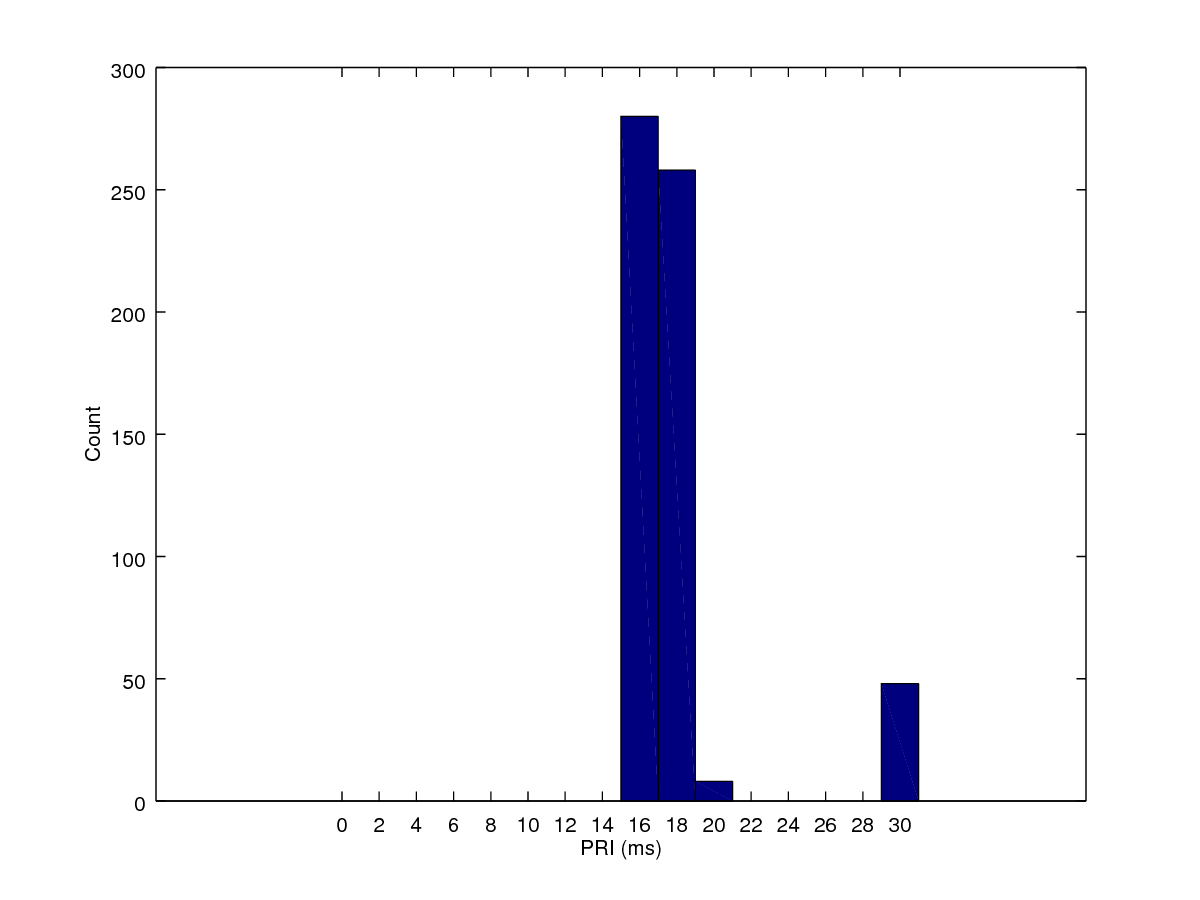
\includegraphics[width=\linewidth]{fig/helloworld_sky.png}
		\subcaption{TelosB PRIs}
	\end{subfigure}
	\begin{subfigure}{0.45\linewidth}
		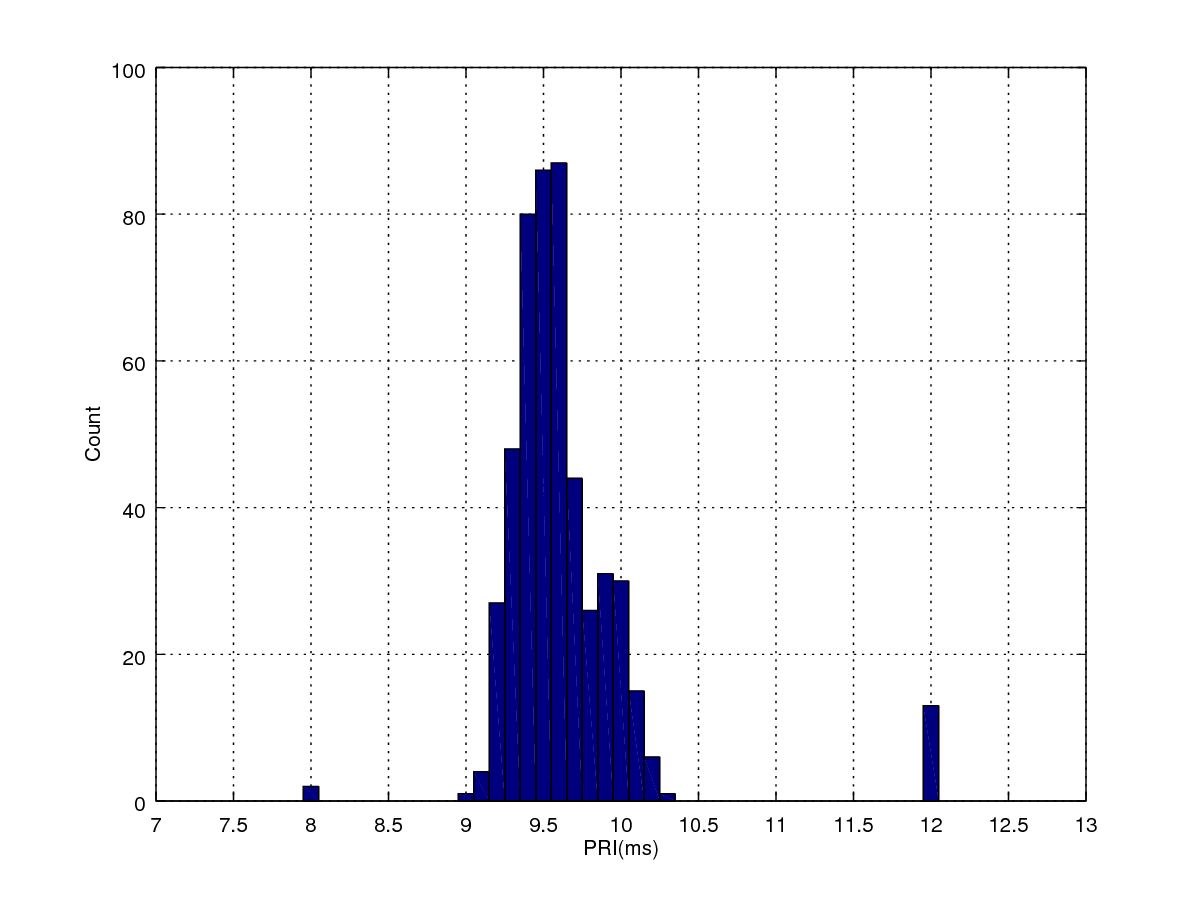
\includegraphics[width=\linewidth]{fig/helloworld_cc2538.png}
		\subcaption{CC2538 PRIs}
	\end{subfigure}
	\caption{PRIs for different devices. \label{PRIs}}
\end{figure}

We also realised that certain outliers exist in our data, represented by the right most bars in \Cref{PRIs}. $13.789$\%  of the PRIs are $\geq$ $18.5$ms on Sky, and $15.307$\% are $\geq$ $11.5$ms on CC2538. A common cause of the outliers is processor being occupied by other tasks when a PING request is received; therefore prolonged the PRI, as illustrated by \Cref{PingloadExample}. The portion of the outlier is hence affected by the payload on the node and the frequency of PING requests. We discuss further details of the outliers in \Cref{PingLoad}.

\subsection{Factors Affecting PRI} \label{PingDevice}

Even though \Cref{PRI_Devices} demonstrated that PRI has a nice distinguishability over our experimented devices, other factors must be taken into account when using PRI as a hint to devices. 

%802.15.4 Security Setting
For example, when 802.15.4 security\cite{802154} is enabled, additional time will be taken for cryptographic operations. PRI can further vary due to different implementations, such as the hardware or software AES implementation on a TelosB. \Cref{802154SecPRI} illustrates a comparison between TelosB SW/HW AES and CC2538 SW AES with 802.15.4 security enabled. In addition, excessive PING frequent could also have an impact to the measured PRI as the flooding packets would overrun the processing power of the low resourced devices.

\begin{figure}[ht!]
	\centering
	\begin{subfigure}{0.4\textwidth}
	{
		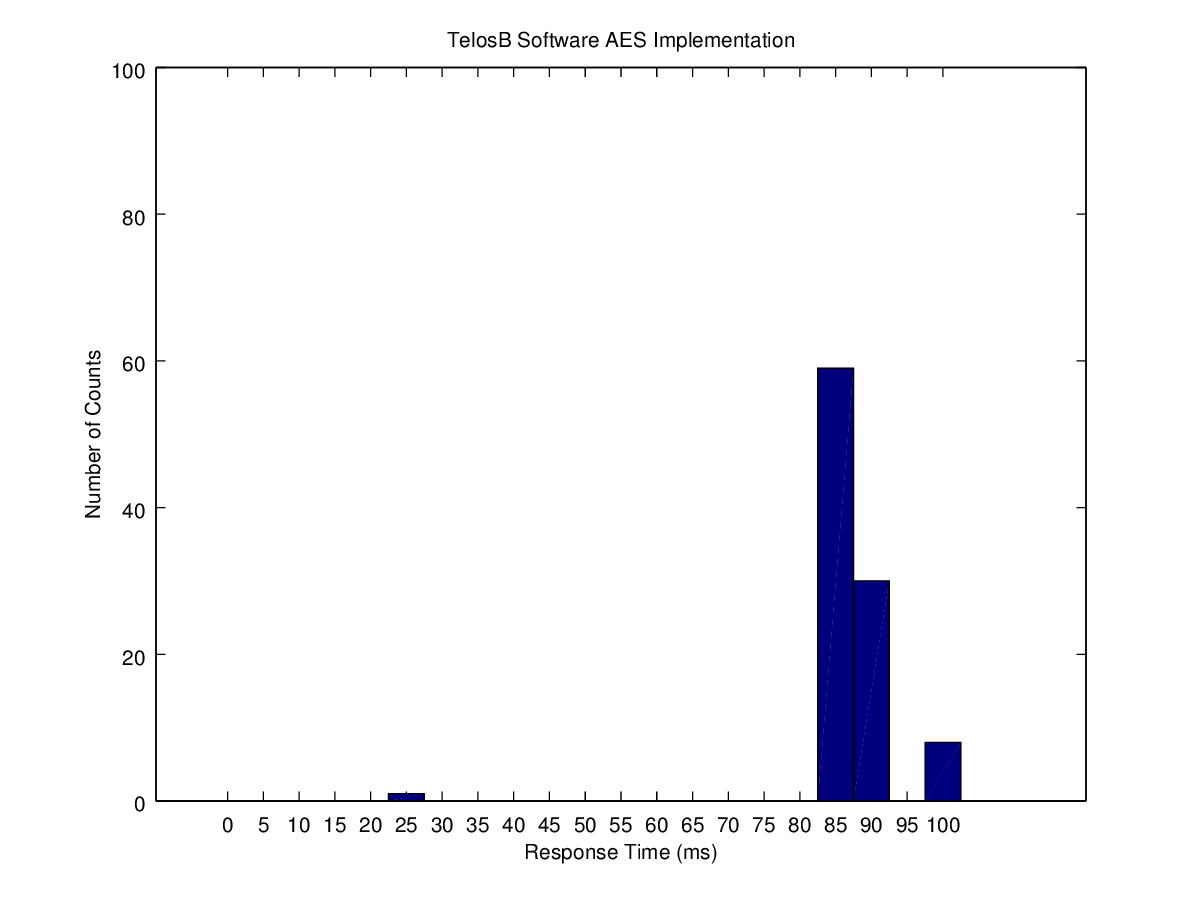
\includegraphics[width=\textwidth]{fig/noncoresec_ping_telosb_sw.png}
	}
	\end{subfigure}
	\begin{subfigure}{0.4\textwidth}
	{
		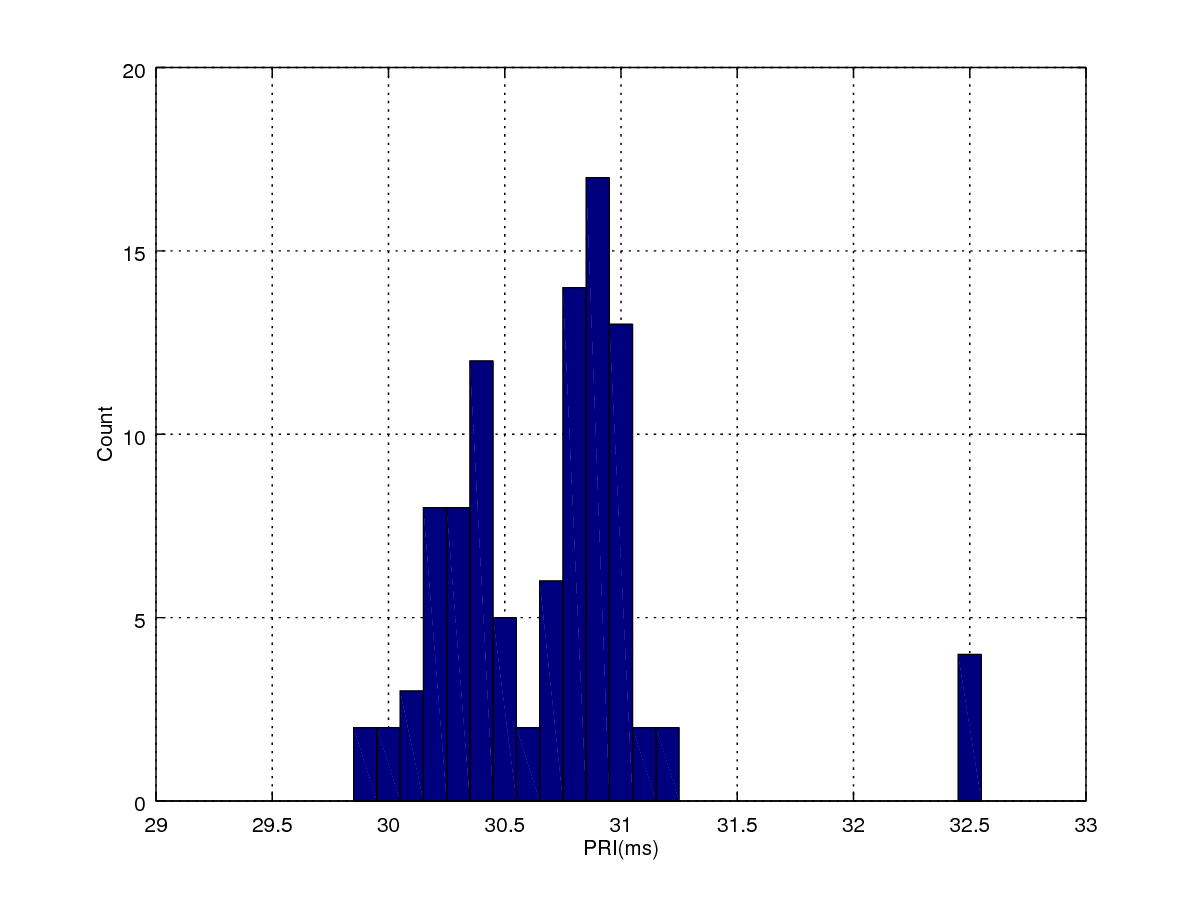
\includegraphics[width=\textwidth]{fig/noncoresec_ping_telosb_hw.png}
	}
	\end{subfigure}
	\begin{subfigure}{0.4\textwidth}
	{
		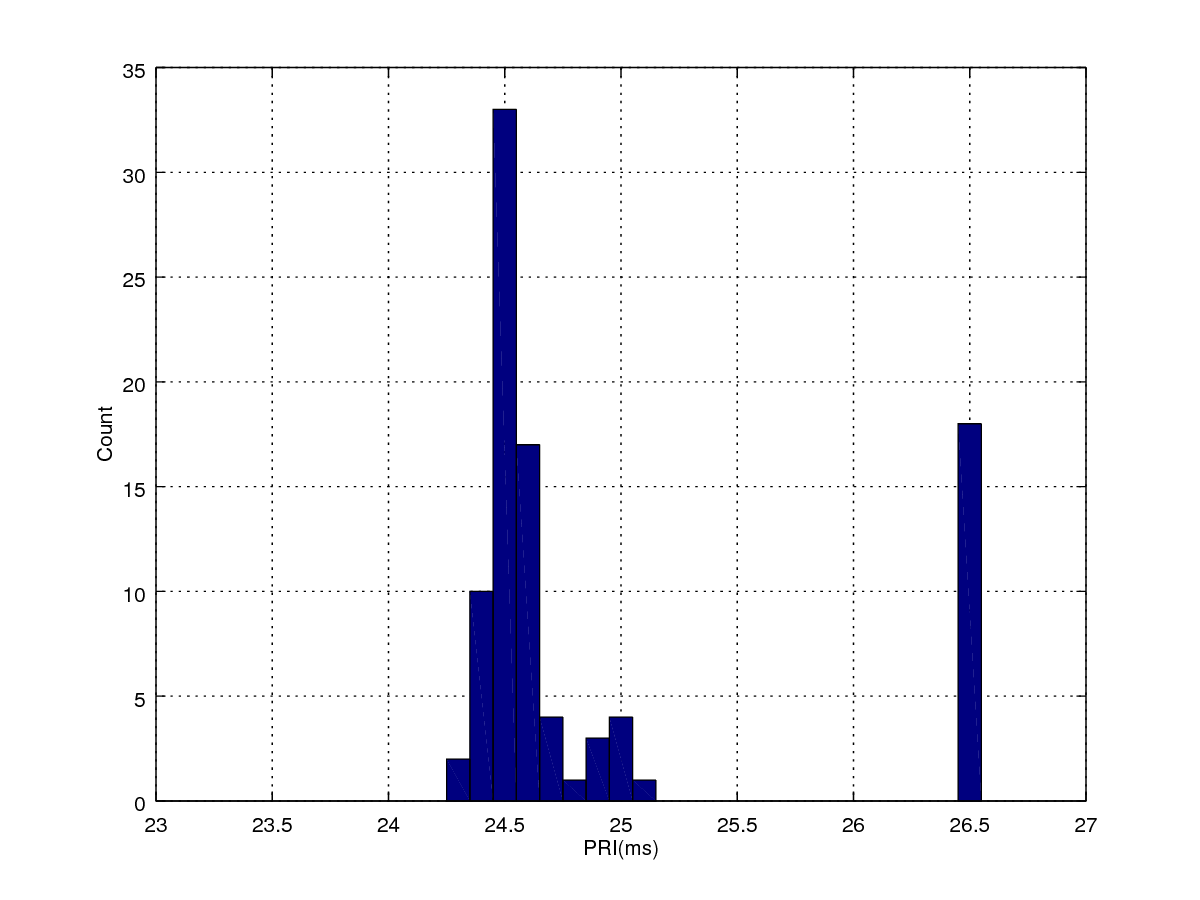
\includegraphics[width=\textwidth]{fig/noncoresec_ping_cc2538_sw.png}
	}
	\end{subfigure}

	\adjustbox{max width = \textwidth}
	{
		\begin{tabular}{|c|c|c|}
			\hline
			              & Mean (ms)     & Median (ms)   \\ \hline
			TelosB HW AES & 37.20 & 30.77 \\ \hline
			TelosB SW AES & 105.19        & 87.40          \\ \hline
			CC2538 SW AES & 48.83         & 24.55          \\ \hline
		\end{tabular}
	}
	
	\caption{PRIs with 802.15.4 security\label{802154SecPRI}}
\end{figure}



